%%%%%%%%%%%%%%%%%%%%%%%%%%%%% Define Article %%%%%%%%%%%%%%%%%%%%%%%%%%%%%%%%%%
\documentclass{article}
%%%%%%%%%%%%%%%%%%%%%%%%%%%%%%%%%%%%%%%%%%%%%%%%%%%%%%%%%%%%%%%%%%%%%%%%%%%%%%%

%%%%%%%%%%%%%%%%%%%%%%%%%%%%% Using Packages %%%%%%%%%%%%%%%%%%%%%%%%%%%%%%%%%%
\usepackage{geometry}
\usepackage{graphicx}
\usepackage{amssymb}
\usepackage{amsmath}
\usepackage{amsthm}
\usepackage{empheq}
\usepackage{mdframed}
\usepackage{booktabs}
\usepackage{lipsum}
\usepackage{graphicx}
\usepackage{color}
\usepackage{psfrag}
\usepackage{pgfplots}
\usepackage{bm}
\usepackage{hyperref}
\hypersetup{
  colorlinks,
  citecolor=black,
  filecolor=black,
  linkcolor=black,
  urlcolor=black
}

\usepackage{fontawesome5}
\usepackage{todonotes}
%%%%%%%%%%%%%%%%%%%%%%%%%%%%%%%%%%%%%%%%%%%%%%%%%%%%%%%%%%%%%%%%%%%%%%%%%%%%%%%

% Other Settings

%%%%%%%%%%%%%%%%%%%%%%%%%% Page Setting %%%%%%%%%%%%%%%%%%%%%%%%%%%%%%%%%%%%%%%
\geometry{a4paper}

%%%%%%%%%%%%%%%%%%%%%%%%%% Define some useful colors %%%%%%%%%%%%%%%%%%%%%%%%%%
\definecolor{ocre}{RGB}{243,102,25}
\definecolor{mygray}{RGB}{243,243,244}
\definecolor{deepGreen}{RGB}{26,111,0}
\definecolor{shallowGreen}{RGB}{235,255,255}
\definecolor{deepBlue}{RGB}{61,124,222}
\definecolor{shallowBlue}{RGB}{235,249,255}
%%%%%%%%%%%%%%%%%%%%%%%%%%%%%%%%%%%%%%%%%%%%%%%%%%%%%%%%%%%%%%%%%%%%%%%%%%%%%%%
%Timeline stuff
\usepackage{etoolbox}
\usepackage{xcolor}
\usepackage{titlesec}
\titleformat{\section}[display]{\bfseries}{\Large\textcolor{gray}{%
    \ifnumcomp{\thesection}{>}{9}{\thesection}{0\thesection}}%
    }{1mm}{\huge}
\usepackage{listings}
\usepackage[most]{tcolorbox}

\newtcolorbox{releaseyear}[2]{%
blanker, breakable, 
     left=5mm, left skip=10.2mm,
     top=-2.2mm,
     coltitle=black,
     attach boxed title to top left={yshift=-12mm, xshift=-13mm},
     fonttitle=\bfseries\Large,
     finish={\draw[#2, line width=3mm,line cap=round]
(frame.south west) -- (frame.north west);},
    title={\rotatebox{90}{#1}}
}
\newtcolorbox{releasequarter}[2]{%
  blanker,  
  left=11mm,top=4mm,
  finish={\draw[#2, line width=3mm,line cap=round]
  (frame.south west) -- (frame.north west);},
  coltitle=#2,
  attach boxed title to top left={yshift=-4mm},
  fonttitle=\bfseries,
  title={#1}
}


\newcommand{\release}[2]{%
        #1
        \hspace*{\fill}
        \textcolor{gray}{#2}\par}

%%%%%%%%%%%%%%%%%%%%%%%%%% Define an orangebox command %%%%%%%%%%%%%%%%%%%%%%%%
\newcommand\orangebox[1]{\fcolorbox{ocre}{mygray}{\hspace{1em}#1\hspace{1em}}}
%%%%%%%%%%%%%%%%%%%%%%%%%%%%%%%%%%%%%%%%%%%%%%%%%%%%%%%%%%%%%%%%%%%%%%%%%%%%%%%

%%%%%%%%%%%%%%%%%%%%%%%%%%%% English Environments %%%%%%%%%%%%%%%%%%%%%%%%%%%%%
\newtheoremstyle{mytheoremstyle}{3pt}{3pt}{\normalfont}{0cm}{\rmfamily\bfseries}{}{1em}{{\color{black}\thmname{#1}~\thmnumber{#2}}\thmnote{\,--\,#3}}
\newtheoremstyle{myproblemstyle}{3pt}{3pt}{\normalfont}{0cm}{\rmfamily\bfseries}{}{1em}{{\color{black}\thmname{#1}~\thmnumber{#2}}\thmnote{\,--\,#3}}
\theoremstyle{mytheoremstyle}
\newmdtheoremenv[linewidth=1pt,backgroundcolor=shallowGreen,linecolor=deepGreen,leftmargin=0pt,innerleftmargin=20pt,innerrightmargin=20pt,]{theorem}{Theorem}[section]
\theoremstyle{mytheoremstyle}
\newmdtheoremenv[linewidth=1pt,backgroundcolor=shallowBlue,linecolor=deepBlue,leftmargin=0pt,innerleftmargin=20pt,innerrightmargin=20pt,]{definition}{Definition}[section]
\theoremstyle{myproblemstyle}
\newmdtheoremenv[linecolor=black,leftmargin=0pt,innerleftmargin=10pt,innerrightmargin=10pt,]{problem}{Problem}[section]
%%%%%%%%%%%%%%%%%%%%%%%%%%%%%%%%%%%%%%%%%%%%%%%%%%%%%%%%%%%%%%%%%%%%%%%%%%%%%%%

%%%%%%%%%%%%%%%%%%%%%%%%%%%%%%% Plotting Settings %%%%%%%%%%%%%%%%%%%%%%%%%%%%%
\usepgfplotslibrary{colorbrewer}
\pgfplotsset{width=8cm,compat=1.9}
%%%%%%%%%%%%%%%%%%%%%%%%%%%%%%%%%%%%%%%%%%%%%%%%%%%%%%%%%%%%%%%%%%%%%%%%%%%%%%%

%%%%%%%%%%%%%%%%%%%%%%%%%%%%%%% Title & Author %%%%%%%%%%%%%%%%%%%%%%%%%%%%%%%%
\title{GSoC 2025: Special Functions in The Julia Programming Language}
\author{Ahmed Y. Kadah$^1$  
\\Oscar D. Smith$^2$ 
\\$^1$ Student, University of Science and Technology in Zewail City
\\ $2$ Mentor, JuliaHub}
\date{}
%%%%%%%%%%%%%%%%%%%%%%%%%%%%%%%%%%%%%%%%%%%%%%%%%%%%%%%%%%%%%%%%%%%%%%%%%%%%%%%

\begin{document}
    \maketitle
    \begin{tikzpicture}[remember picture,overlay]
    \node[anchor=north west,yshift=-1.5pt,xshift=1pt]%
        at (current page.north west)
        {
\includegraphics[height=20mm]{images/gsoc logo}};
    \end{tikzpicture}

    \begin{tikzpicture}[remember picture,overlay]
    \node[anchor=north west,yshift=-1.5pt,xshift=60pt]%
        at (current page.north west)
        {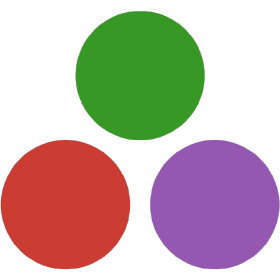
\includegraphics[height=20mm]{images/julia logo 2}};
    \end{tikzpicture}

  \section*{Abstract}
    In this project, we will work on implementing high speed and high accuracy implementations of various special functions, as well as optimizing and improving existing implementations in Julia.
    Our work will mostly be on the SpecialFunctions.jl Julia library but will touch on some of the issues in the HyperGeometricFunctions.jl library as well. 
    \todo{Improve the abstract}

  \section*{Introduction}
    \subsection*{About me 
      \href{https://github.com/AhmedYKadah}{\faGithub}    
      \href{https://linkedin.com/in/ahmed-yasser-kadah-83687b269}{\faLinkedin}    
      \href{mailto:ahmadyassermo@gmail.com}{\faEnvelope[regular]}    
    }\label{sub:About} 
      Hi there! I am Ahmed Yasser Kadah, a third year Communications and Information Engineering student at the University of Science and Technology in Zewail City, Giza, Egypt.
      I recently took an advanced course in partial differential equations and special functions, so when I saw this project I thought it would be interesting to follow along this path and study the topics further when it comes to real world applications and make something that would genuinely benefit others. 
      This is my first time contributing to an open source project and just recently made my first contribution with a pull request for a Julia implementation of the Float64 erf(x) (will be explained later). \cite{pr} 





    \subsection*{Background on Special Functions}\label{sub:Background } % (fold)
    Special functions are a class of mathematical functions that arise in the solutions of complex physical, engineering, and mathematical problems.\cite{special functions}
   These functions are typically defined by specific properties or satisfy particular differential equations, and they include some of the most well-known functions in mathematics, such as the error function, Gamma function, and Bessel functions.

   This class of functions serve a unique purpose in many different applications, as they have properties which can be utilized to solve highly complex problems which otherwise have no analytic solutions, or even assist in numerical computation.


    Due to the nature and importance of this topic, there already exists a large number of implementations in other languages such as Wolfram Mathematica, MATLAB, and many more.
    However, the number of memory efficient and open source implementations are somewhat limited to languages like C. 
    \todo{Reword this}
    Hence, our aim here is not to reinvent the wheel, but refine it. 

    SpecialFunctions.jl and HyperGeometricFunctions.jl are Julia libraries which aim to provide Julia implementations/interfaces for special functions.
    While HyperGeometricFunctions.jl is purely implemented in julia, SpecialFunctions.jl makes use of external libraries like openlibm and openspecfun which adds a layer of overhead and reduces the efficiency.
    \todo{Add Part about compatibility of julia implementations with auto diff, and explain what autodiff is}



    
    % subsection* Background  (end)
    \subsection*{Goals}\label{sub:Goals} % (fold)
    \todo{Cover more ideas and issues}
    \todo{Go into more detail about SpecialFunctions.jl and HyperGeometricFunctions.jl and what exactly is going to be done, then add the specifics in the deliverables}
      The goals of the project are to (1) implement some of the functions which currently use external library calls in Julia, (2) work on fixing some of the existing issues in the github repositories, (3) optimizing poorly optimized implementations, (4) explore and add missing functions. 

      The implementations of functions will make use of different methods  of numerical approximation methods like polynomial/rational approximation. 
      Some of the important tools include: \begin{enumerate}
        \item Remez.jl, a library for constructing minimax polynomials and rational functions 
        \item Sollya, another powerful tool for constructing polynomials but with a less convenient interface. Will be used as the reference for the performance of Remez.jl and possibly some contributions.
      \end{enumerate}
      \todo{give proper description of each}
    
    % subsection* Literature Review (end)
  \section*{Deliverables and Timeline}\label{sec:Methods} % (fold)
    \subsection*{Deliverables}
    \todo{Break down each deliverable into what exactly is being delivered, ex. the definition of the error function, what are the targeted data types, etc.}
      \begin{itemize}
        \item Fully implemented \href{https://github.com/JuliaMath/SpecialFunctions.jl/blob/master/src/erf.jl}{\textbf{error function}} and it's varieties \cite{error function}
          \begin{itemize}
            \item Error Function: $\operatorname{erf } (x)=\frac{2 }{\sqrt{\pi } }\int_{0}^{x} e ^{-t^2}\text{d}t$ for Float32, and BigFloat (Float64 has been implemented as said previously), for real as well as complex inputs.
            \item Complementary Error Function: $\operatorname{erfc } (x)=1- \frac{2 }{\sqrt{\pi } }\int_{0}^{x} e ^{-t^2}\text{d}t$ for Float32, Float64, and BigFloat, for real as well as complex inputs.
            \item Scaled Complementary Error Function: $\operatorname{erfcx } (x)=e ^{x^2 } \operatorname{erfc} (x)$ for Float32, Float64, and BigFloat, for real as well as complex inputs.
            \item Imaginary Error Function: $\operatorname{erfi } (x)= -i \operatorname{erf} (ix)$ for Float32, Float64, and BigFloat, for real as well as complex inputs.
            \item Dawson Function: $D (x)=\frac{\sqrt{\pi } }{2 }e ^{-x^2 } \operatorname{erfi} (x)$ for Float32, Float64, and BigFloat, for real as well as complex inputs.
            \item Faddeeva Function: $w (z)=e ^{-z^2 } \operatorname{erfi} (z)= \operatorname{erfcx}(-iz)$ for Float32, Float64, and BigFloat, for complex inputs.
          \end{itemize}
        % \item Implementation of \href{https://github.com/JuliaMath/SpecialFunctions.jl/blob/master/src/gamma.jl}{gamma function} for real and complex inputs. 
        \item At least 15 issues resolved on \href{https://github.com/JuliaMath/SpecialFunctions.jl/issues}{\textbf{SpecialFunctions.jl}} 
        \item At least 5 issues resolved on \href{https://github.com/JuliaMath/HypergeometricFunctions.jl/issues}{\textbf{HyperGeometricFunctions.jl}} 
        \item Implementation of Appel Hypergeometric Function \cite{appell} 
          \begin{itemize}
            \item $F_1 $ is defined for $\lvert x  \rvert <1 $, $\lvert y  \rvert < 1 $ by the series \[
              F_1(a,b_1,b_2;c;x,y)=\displaystyle\sum_{m,n=0 }^{\infty } \displaystyle\frac{(a)_{m+n }(b_1)_{m }(b_2)_{n }}{(c)_{m+n}m!n! }x ^m y^n 
            \] 
              where $(q)_n $ is the Pochhammer symbol.
            \item $F_2 $ is defined for $\lvert x  \rvert +\lvert y  \rvert < 1 $ by the series \[
              F_2(a,b_1,b_2;c_1,c_2;x,y)=\displaystyle\sum_{m,n=0 }^{\infty } \displaystyle\frac{(a)_{m+n }(b_1)_{m }(b_2)_{n }}{(c_1)_{m}(c_2)_{n}m!n! }x ^m y^n 
            \] 
            \item $F_3 $ is defined for $\lvert x  \rvert <1 $, $\lvert y  \rvert < 1 $ by the series \[
              F_3(a_1,a_2,b_1,b_2;c;x,y)=\displaystyle\sum_{m,n=0 }^{\infty } \displaystyle\frac{(a_1)_{m}(a_2)_{n}(b_1)_{m }(b_2)_{n }}{(c)_{m+n}m!n! }x ^m y^n 
            \] 
            \item $F_4 $ is defined for $\lvert x  \rvert ^{1/2} +\lvert y  \rvert ^{1/2}< 1 $ by the series \[
              F_4(a,b;c_1,c_2;x,y)=\displaystyle\sum_{m,n=0 }^{\infty } \displaystyle\frac{(a)_{m+n }(b)_{m+n }}{(c_1)_{m}(c_2)_{n}m!n! }x ^m y^n 
            \] 
          \end{itemize}
      \end{itemize}
    \subsection*{Timeline}
    \todo{Finish Timeline}
      \begin{releaseyear}{June '25}{cyan}
        \begin{releasequarter}{W 1}{cyan!50}
          \release{}{}
        \end{releasequarter}
        \begin{releasequarter}{W 2}{cyan!50}
          \release{}{}
        \end{releasequarter}
        \begin{releasequarter}{W 3}{cyan!50}
          \release{}{}
        \end{releasequarter}
        \begin{releasequarter}{W 4}{cyan!50}
          \release{}{}
        \end{releasequarter}
      \end{releaseyear}
      \begin{releaseyear}{July '25}{teal}
        \begin{releasequarter}{W 1}{teal!50}
          \release{}{}
        \end{releasequarter}
        \begin{releasequarter}{W 2}{teal!50}
          \release{}{}
        \end{releasequarter}
        \begin{releasequarter}{W 3}{teal!50}
          \release{}{}
        \end{releasequarter}
        \begin{releasequarter}{W 4}{teal!50}
          \release{}{}
        \end{releasequarter}
      \end{releaseyear}
      \begin{releaseyear}{August '25}{orange}
        \begin{releasequarter}{W 1}{orange!50}
          \release{}{}
        \end{releasequarter}
        \begin{releasequarter}{W 2}{orange!50}
          \release{}{}
        \end{releasequarter}
        \begin{releasequarter}{W 3}{orange!50}
          \release{}{}
        \end{releasequarter}
        \begin{releasequarter}{W 4}{orange!50}
          \release{}{}
        \end{releasequarter}
      \end{releaseyear}
  
  % section* Methods (end)
  \section*{Expected Results}\label{sec:Results} % (fold)
    Complete, functional, high efficiency and accuracy, julia implementations of the following:
    \todo{Finish this or make it into expected difficulties or things along that line}
  
  % % section* References (end)
  % \section*{References}\label{sec:References} % (fold)
    
    \begin{thebibliography}{9}
      \bibitem{pr}
      \url{https://github.com/JuliaMath/SpecialFunctions.jl/pull/491}

      \bibitem{special functions}
      \url{https://en.wikipedia.org/wiki/Special_functions}  

      \bibitem{hypergeometric functions}
      \url{https://en.wikipedia.org/wiki/Hypergeometric_function}

      \bibitem{error function}
      \url{https://en.wikipedia.org/wiki/Error_function}

      \bibitem{SpecialFunctions.jl}
      \url{https://github.com/JuliaMath/SpecialFunctions.jl}

      \bibitem{HypergeometricFunctions.jl}
      \url{https://github.com/JuliaMath/HypergeometricFunctions.jl}

      \bibitem{wolfram special functions}
      \url{https://reference.wolfram.com/language/guide/SpecialFunctions.html.en}

      \bibitem{wolfram hypergeometric}
      \url{https://reference.wolfram.com/language/guide/HypergeometricFunctions.html}

      \bibitem{matlab special functions}
      \url{https://www.mathworks.com/help/matlab/special-functions.html}

      \bibitem{matlab hypergeometric}
      \url{https://www.mathworks.com/help/symbolic/sym.hypergeom.html}

      \bibitem{scipy}
      \url{https://docs.scipy.org/doc/scipy/reference/special.html}

      \bibitem{gsl}
      \url{https://www.gnu.org/software/gsl/}

      \bibitem{ForwardDiff.jl}
      \url{https://github.com/JuliaDiff/ForwardDiff.jl}

      \bibitem{remez.jl}
      \url{https://github.com/simonbyrne/Remez.jl}

      \bibitem{sollya}
      \url{https://www.sollya.org/}

      \bibitem{remez}
      \url{https://en.wikipedia.org/wiki/Remez_algorithm}

      \bibitem{appell}
      \url{https://en.wikipedia.org/wiki/Appell_series}
    \end{thebibliography}
    \todo{Finish all citations}
  
  % section* References (end)
\end{document}
